% Provenance (never printed): old premiere S material on the history of plate
% tectonics (from continental drift to seafloor spreading: the ridges, the
% magnetic stripes, the ages of the drilled floor); see
% sources/book2/PROVENANCE.md. Profiles are computed in
% figdata/grade-11/magnetic_stripes.py, the age map in seafloor_age.py, the
% drilling fit in sediment_ages.py.
\chapter{从大陆漂移到海底扩张}\label{ch:g11:drift-to-spreading}

20 世纪 50 年代初，在哥伦比亚大学的拉蒙特实验室，一位年轻的
地质学家玛丽·瑟普坐在一排排长长的数字前。每个数字都是北大西洋的一个水深，
由船上的回声测深仪测得，沿船只的航迹依次排列，
她将它们逐一绘制成图，描绘出沿
曾横渡大洋的船只航迹的海底形状。大洋中央，海底隆起，
成为一道山脉——在每条航迹上，沿山脊顶部，
海底又陡然下陷，形成一道深深的裂隙，仿佛山脉已被从中间劈开。
本章讲述这类洋底测量
如何将一个曾被否定的想法——大陆漂移，发展为一种理论：洋底
在洋脊处生成，并从洋脊向两侧扩展，其岩石中保存着
洋底自身年龄的记录。
% ledger: aip:tharp, aip:featureless, usgs:echo-sounding

\begin{recall}
大陆漂移是指大陆会移动的观点；阿尔弗雷德·魏格纳
自 1912 年起为之辩护，依据是海岸线的吻合、化石、岩石和古气候，
但无法说明是什么使大陆移动。地球表面由刚性板块构成，
这些板块在离散型、汇聚型和转换型边界处相接；
它们每年移动几厘米，每年 $\qty{1}{cm}$ 相当于
每百万年 $\qty{10}{km}$（第 1 册，七年级）。海底有其大陆架，
\omterm{def:g10:layered-ocean:thermocline}{深海}平原、洋脊和海沟（第 1 册，八年级）。
地球具有磁场，有南北两个磁极，
指南针的指针随之指向；声脉冲射入水中，以回声形式返回，
所经历的时间可给出距离（见物理学分册）。
\end{recall}

\section{大陆漂移为何被否定}

魏格纳的证据表明，大陆曾经是相连的。然而，它
并未说明大陆如何能够移动。魏格纳设想大陆
在洋底岩石中犁行，而物理学家回答说，已知的任何力都无法推动大陆穿过坚硬的岩石
而不将其压碎。半个世纪以来，大多数地质学家认为
大陆根本没有移动过。
% ledger: usgs:wegener-1912, usgs:jeffreys (Book 1 rows)

当时缺少两样东西。第一是一种机制。第二样东西
也是引出第一样的，是对洋底的认识。洋底覆盖了地球的大部分
表面，而在 1912 年，几乎没有人见过它：人们以为它
是一片几乎没有任何特征的平原。
% ledger: aip:tharp, aip:featureless

\section{绘制洋底地图}

回声测深仪从船体向海底发出一个短促的声脉冲，
并记录其回声的时间。声音在海水中的速度约为
\qty{1500}{m/s}；脉冲向下再返回，因此延迟 $t$ 对应一个
深度
\[
  d = \frac{v\,t}{2}.
\]
例如，\qty{6.0}{s} 的延迟对应 $1500 \times 6.0/2 =
\qty{4500}{m}$ 的水深。十九世纪，水深是
逐点测量，即将带重物的测绳放到海底。第一次世界大战后，
回声测深仪取而代之，其回声记录显示海底
远比人们想象的崎岖；20 世纪 50 年代，多国船只的测量表明，一条
巨大的海底山脉几乎环绕整个
地球。
% ledger: noaa:sound-seawater, usgs:echo-sounding, usgs:line-soundings

\begin{history}[玛丽·瑟普与裂谷，1952]
% ledger: aip:tharp, aip:featureless
1947 年起，地球物理学家布鲁斯·希泽恩已收集了北大西洋各处的回声测深剖面。
玛丽·瑟普当时不被允许登上科考船，
她把自己后来称之为“无尽的测深数字行”的东西，
绘成了海底图。1952 年，她将东西向航线按由北至南的顺序排列，
发现有一个地貌特征在各条航线间都能对应：
沿大西洋中脊脊顶的一道裂隙，即
裂谷。希泽恩起初以为这是误差；随后，
将大西洋地震的震中按相同比例尺标出，发现它们
正落在裂谷之中。瑟普与希泽恩绘制的世界洋底图，
由画家海因里希·贝伦于 1977 年绘制，首次让人们看到了洋底的真实面貌；1997 年，
国会图书馆将她评为
二十世纪四位伟大的制图师之一。
\end{history}

洋中脊构成一个几乎连续的整体系统，
全长约 \qty{65000}{km}，其中九成以上位于水下；脊顶
平均位于海面以下 \qty{2500}{m}。沿扩张缓慢的大西洋中脊，
脊顶被裂谷切割；沿扩张较快的东太平洋海隆，脊顶则是
一道平缓光滑的山顶。大洋中的地震与洋脊
紧密相随。一切迹象都指向洋脊是一个
正在发生某种变化的地方——但究竟是什么？
% ledger: noaa:ridge, aip:tharp

\section{海底扩张}

\begin{history}[赫斯与传送带，1962]
% ledger: usgs:hess, hess:1962
1962 年，哈里·赫斯是普林斯顿大学的地质学家，同时也是海军预备役将官，
出版了 \emph{History of Ocean Basins}。
他提出，热岩石在洋脊之下上升，形成新的洋底，
随后像传送带一样向两侧移开，并在
海沟处重新没入地幔。罗伯特·迪茨也得出了同样的想法，并为其命名：
\omterm{def:g11:drift-to-spreading:spreading}{海底扩张}。这一想法解释了为何地球不会变大，
尽管新的洋底不断生成；为何洋底的沉积物如此之少，
以及为何洋底岩石远比
大陆岩石年轻。
\end{history}

\begin{definition}[海底扩张]\label{def:g11:drift-to-spreading:spreading}
\emph{海底扩张}\index{海底扩张}是一个过程，通过这一过程
新的洋底沿洋中脊的脊顶形成，那里的熔融岩石
从地幔上升并固结，随后向洋脊两侧移开，使洋底的年龄
随离洋脊距离的增加而增大。
\end{definition}

\begin{definition}[扩张速率]\label{def:g11:drift-to-spreading:spreading-rate}
洋脊的\emph{全扩张速率}\index{全扩张速率}是指
洋脊两侧两块板块相互远离的速度。\emph{半扩张速率}
是指洋脊一侧的洋底远离洋脊
轴线的速度。若扩张对称，则全扩张速率为半扩张速率的两倍。
\end{definition}

各洋脊的扩张速度差异很大。大西洋中脊的张开速度为
\qtyrange{2}{5}{cm}每年，东太平洋海隆则为\qtyrange{6}{16}{cm}
每年。现有洋底中，约三分之一形成于慢速洋脊
（\omterm{def:g11:drift-to-spreading:spreading-rate}{全扩张速率}为\qtyrange{20}{55}{mm}每年），约五分之二则形成于
快速洋脊（\qtyrange{75}{180}{mm}每年）。
% ledger: noaa:ridge, seton:rate-classes

赫斯的设想大胆，起初几乎没有直接证据。证据
来自两个出人意料的方面：洋底的磁性及其
沉积物。

\section{地磁倒转与条带状海底}

\subsection{岩石记录了磁场}

洋底玄武岩中含有少量磁铁矿颗粒，磁铁矿是一种
铁氧化物，具有强磁性。玄武岩熔岩喷发时温度极高，
不可能保留任何持久的磁化；冷却时，颗粒被
磁化，其方向与周围的地球磁场平行，并随之
锁定在岩石中。
% ledger: usgs:magnetometers

\begin{definition}[剩余磁化；居里温度]\label{def:g11:drift-to-spreading:remanence}
磁性矿物的\emph{居里温度}\index{居里温度}是
即超过此温度便无法保持自身磁化强度的温度，磁铁矿约为
\qty{580}{\celsius}。岩石中的磁性颗粒若在地球磁场中冷却并越过
其居里温度，则保留与当时磁场平行的磁化强度，
即当时磁场的方向，这种磁化称为
\emph{剩余磁化}\index{剩余磁化}。该磁化在磁场改变后仍能长期保持，除非岩石
再次被加热至居里温度以上。
\end{definition}
% ledger: tarduno:curie

\begin{omfigure}
\begin{tikzpicture}[font=\footnotesize, >={Stealth[length=5pt]}]
  % ground and lava flow
  \fill[lith basalt] (0,0) rectangle (11,0.6);
  \fill[omLithBasalt!45!red!35] (0,0.6) -- (11,0.6) -- (11,1.9) .. controls (9,2.0) and (4,2.15) .. (0,2.05) -- cycle;
  \fill[omLithBasalt!70] (0,1.35) -- (11,1.25) -- (11,1.9) .. controls (9,2.0) and (4,2.15) .. (0,2.05) -- cycle;
  \draw[black!60] (0,1.35) -- (11,1.25);
  \draw[line width=0.8pt] (0,2.05) .. controls (4,2.15) and (9,2.0) .. (11,1.9);
  \draw[black!60] (0,0.6) -- (11,0.6);
  % field lines (northern hemisphere: pointing down to the north)
  \foreach \x in {0.6,2.4,4.2,6.0,7.8,9.6} {
    \draw[->, omDef, line width=0.9pt] (\x,4.0) -- (\x+1.1,2.55);
  }
  \node[anchor=south west, text=omDef] at (0.2,4.05) {地球磁场};
  % locked grains in the cooled top
  \foreach \x in {0.5,1.3,...,10.5} {
    \draw[->, black, line width=0.6pt] (\x,1.86) -- (\x+0.25,1.53);
  }
  % random grains in the hot interior
  \foreach \x/\a in {0.6/20,1.5/140,2.3/250,3.2/80,4.0/310,4.9/190,5.7/40,6.6/120,7.4/280,8.3/20,9.1/200,10.0/330} {
    \draw[->, black!55, line width=0.5pt] (\x,0.95) -- ++(\a:0.22);
  }
  \node[anchor=west, align=left] at (11.15,1.75) {冷却至 \qty{580}{\celsius} 以下：\\颗粒保留磁场方向};
  \node[anchor=west, align=left] at (11.15,0.92) {仍高于 \qty{580}{\celsius}：\\无持久磁化};
  \node[anchor=west, align=left] at (11.15,0.25) {较老的岩石};
  \node[anchor=west] at (9.0,4.25) {北 $\rightarrow$};
\end{tikzpicture}

{\small 熔岩流冷却示意图（北半球，磁场
指向北方并向下）。熔岩流顶部已冷却至磁铁矿的
\omterm{def:g11:drift-to-spreading:remanence}{居里温度}以下：其磁性颗粒（黑色箭头）保持
磁场方向。内部温度仍较高，尚未记录任何信息；它
将在冷却时记录当时的磁场。}
\end{omfigure}

\subsection{磁场发生倒转}

二十世纪初，布伦（1906 年）和随后的松山基范
（1920 年代）发现火山岩可分为两组。其中
一些的磁化方向与现今磁场一致；另一些则
的磁化方向相反，仿佛南北磁极已互换
位置。磁场本身曾反复倒转。
% ledger: usgs:reversals

\begin{definition}[地磁倒转；正极性与反极性]\label{def:g11:drift-to-spreading:reversal}
\emph{地磁倒转}\index{地磁倒转}是指地球南北磁极的
互换。磁场指向与今日相同的时期，
称为\emph{正极性}\index{正极性}时期；磁场指向相反的时期，
称为\emph{反极性}\index{反极性}时期。
在任一时期磁化的岩石，
其极性与该时期相同。
\end{definition}

经测年的熔岩给出了正、\omterm{def:g11:drift-to-spreading:reversal}{反极性}时段的序列，即
\emph{地磁极性时间尺度}。其中的长时段以
研究地球磁场的科学家命名（布伦、松山基范、高斯、
吉尔伯特）；其中的短时事件则以
首次发现它们的地点命名。

\begin{omfigure}
\begin{tikzpicture}
\begin{axis}[width=0.92\linewidth, height=3.2cm, xmin=0, xmax=5.5, ymin=-0.9, ymax=1.9,
  axis y line=none, axis x line*=bottom, xtick={0,0.5,...,5.5}, tick label style={font=\small},
  xlabel={年龄（百万年）}, label style={font=\small}, clip=false]
\addplot[fill=black, draw=none] table {figdata/out/grade-11-magnetic_stripes-timescale.dat};
\draw[black] (axis cs:0,0) rectangle (axis cs:5.5,1);
\begin{scope}[every node/.style={font=\scriptsize, anchor=south}]
  \node at (axis cs:0.39,1.05) {布伦};
  \node at (axis cs:1.68,1.05) {松山基范};
  \node at (axis cs:3.08,1.05) {高斯};
  \node at (axis cs:4.74,1.05) {吉尔伯特};
\end{scope}
\draw[black!60] (axis cs:0.78,1) -- (axis cs:0.78,1.45);
\draw[black!60] (axis cs:2.581,1) -- (axis cs:2.581,1.45);
\draw[black!60] (axis cs:3.58,1) -- (axis cs:3.58,1.45);
\begin{scope}[every node/.style={font=\scriptsize, anchor=north}]
  \node at (axis cs:1.03,-0.05) {哈拉米洛};
  \node at (axis cs:1.86,-0.05) {奥杜威};
\end{scope}
\node[font=\scriptsize, anchor=west] at (axis cs:5.55,0.75) {正极性};
\node[font=\scriptsize, anchor=west] at (axis cs:5.55,0.25) {（黑色）};
\end{axis}
\end{tikzpicture}

{\small 过去 550 万年的地磁极性时间尺度：
黑色表示\omterm{def:g11:drift-to-spreading:reversal}{正极性}，白色表示\omterm{def:g11:drift-to-spreading:reversal}{反极性}。当前的\omterm{def:g11:drift-to-spreading:reversal}{正极性}时段
始于 \num{780000} 年前；过去
五百万年内发生过二十次\omterm{def:g11:drift-to-spreading:reversal}{地磁倒转}。数据：Cande 和 Kent（1995）。}
\end{omfigure}
% ledger: ck95:chrons

\subsection{洋底的条纹}

从 1950 年代起，船只拖着磁力计穿越大洋，
发现海面处的磁场并不是预期中来自地核的平滑磁场：
此处略强，彼处略弱。
% ledger: usgs:magnetometers

\begin{definition}[磁异常]\label{def:g11:drift-to-spreading:anomaly}
在海面上的某一点，
\emph{磁异常}\index{磁异常}是该处实测磁场强度减去仅由地球磁场
在该处所应有的强度之差。下方岩石的磁化使磁场增强时为正，
削弱时为负。它与磁场本身相比很小，
以纳特斯拉（\unit{nT}）为单位测量。
\end{definition}

在大范围内绘制\omterm{def:g11:drift-to-spreading:anomaly}{磁异常}时，异常形成了与洋脊脊顶平行的
条纹，正负交替，宛如斑马的皮毛——而洋脊一侧的图样
与另一侧的图样互为镜像。
% ledger: usgs:magnetometers

\begin{history}[瓦因与马修斯，1963 年]
% ledger: vm:1963, usgs:magnetometers
1963 年 9 月，弗雷德·瓦因和德拉蒙德·马修斯在期刊 \emph{Nature} 上发表短文，
题为 \emph{Magnetic anomalies over oceanic ridges}。他们把赫斯的\omterm{def:g11:drift-to-spreading:spreading}{海底扩张}
与磁场倒转结合在一起：若新洋底在脊顶形成并向外移动，
而磁场同时倒转，则每条洋底带都记录了其冷却时的极性。
洋底因此成为一条条纹磁带，在洋脊两侧同时展开：
正常极性条带上方为正异常，\omterm{def:g11:drift-to-spreading:reversal}{反极性}条带上方为负异常，
两侧序列相同。
\end{history}

\begin{omfigure}
\begin{tikzpicture}
\begin{axis}[hide axis, axis equal image, width=0.94\linewidth, xmin=-320, xmax=420, ymin=-120, ymax=160, clip=false]
  % block faces
  \fill[white] (axis cs:-300,0) -- (axis cs:300,0) -- (axis cs:390,70) -- (axis cs:-210,70) -- cycle;
  \fill[omLithBasalt!25] (axis cs:-300,0) rectangle (axis cs:300,-60);
  \fill[omLithBasalt!45] (axis cs:300,0) -- (axis cs:390,70) -- (axis cs:390,10) -- (axis cs:300,-60) -- cycle;
  \addplot[fill=black!80, draw=none] table {figdata/out/grade-11-magnetic_stripes-block.dat};
  \draw[black] (axis cs:-300,0) -- (axis cs:300,0) -- (axis cs:390,70) -- (axis cs:-210,70) -- cycle;
  \draw[black] (axis cs:-300,0) -- (axis cs:-300,-60) -- (axis cs:300,-60) -- (axis cs:300,0);
  \draw[black] (axis cs:300,-60) -- (axis cs:390,10) -- (axis cs:390,70);
  % ridge axis
  \draw[omRidge, line width=1.6pt] (axis cs:0,0) -- (axis cs:90,70);
  \node[font=\footnotesize, text=omRidge, anchor=south] at (axis cs:90,72) {洋脊轴};
  % rising magma
  \fill[red!60!orange, opacity=0.75] (axis cs:-12,-60) -- (axis cs:12,-60) -- (axis cs:3,0) -- (axis cs:-3,0) -- cycle;
  \draw[->, >={Stealth[length=5pt]}, red!70!black, line width=1pt] (axis cs:0,-95) -- (axis cs:0,-62);
  \node[font=\footnotesize, anchor=north] at (axis cs:0,-96) {熔融岩石上升};
  % spreading arrows
  \draw[->, >={Stealth[length=6pt]}, line width=1.2pt] (axis cs:-90,100) -- (axis cs:-220,100);
  \draw[->, >={Stealth[length=6pt]}, line width=1.2pt] (axis cs:150,100) -- (axis cs:280,100);
  \node[font=\footnotesize, anchor=south] at (axis cs:-155,103) {较老};
  \node[font=\footnotesize, anchor=south] at (axis cs:215,103) {较老};
  % legend
  \fill[black!80] (axis cs:-300,-100) rectangle (axis cs:-280,-88);
  \node[font=\footnotesize, anchor=west] at (axis cs:-276,-94) {正极性};
  \draw[black] (axis cs:-300,-118) rectangle (axis cs:-280,-106);
  \node[font=\footnotesize, anchor=west] at (axis cs:-276,-112) {反极性};
\end{axis}
\end{tikzpicture}

{\small 条纹状洋底（示意图，按洋脊两侧各以
\qty{7.5}{cm} 每年的速率扩张计算，时段为过去 400 万年）。每条洋底带
在轴部冷却时保留了当时磁场的极性；
一侧的图样与另一侧互为镜像。}
\end{omfigure}

\begin{proposition}[条纹距洋脊轴的距离]\label{prop:g11:drift-to-spreading:stripe}
若洋脊以恒定的半扩张速率 $u$ 对称扩张，则
于时间 $t$ 之前在轴部形成的洋底，现位于距离
\[
  x = u\,t
\]
处，且位于洋脊轴两侧。特别地，
两条条纹之间记录年龄为 $t$ 的倒转的边界，位于两侧距离 $u\,t$ 处。
\end{proposition}

\begin{proof}
在时间 $t$ 之前于轴部形成的一块洋底，此后
一直以速度 $u$ 远离轴线，历时 $t$，共移动了距离
$u\,t$。在轴的另一侧同一时刻形成的一块洋底，向相反方向
以相同速度运动，并位于相同距离处。反转边界两侧的洋底
分别形成于倒转之前与之后，
因此边界位于年龄为 $t$ 的洋底所在之处，即距离 $u\,t$ 处。
\end{proof}

\omterm{def:g11:drift-to-spreading:anomaly}{磁异常}可由时间尺度计算得出。在下面的剖面图中，
磁化层为一层厚 \qty{1}{km} 的岩层，其顶面位于
海面以下 \qty{3}{km} 处，并按上述命题划分为正、\omterm{def:g11:drift-to-spreading:reversal}{反极性}的块体，
各块体在海面处的磁场被
逐一相加。在宽条带上方，异常在其边缘（即极性变化处）最强，中部较弱；
但异常的符号
取决于下方条带的极性。

\begin{omfigure}
\begin{tikzpicture}
\begin{axis}[omrecord, name=fast, width=0.92\linewidth, height=5.0cm, xmin=-375, xmax=375, ymin=-820, ymax=560,
  ytick={-400,0,400}, xtick={-300,-200,...,300}, tick label style={font=\small}, label style={font=\small},
  ylabel={磁异常 (\unit{nT})}, title={\small 快速洋脊：半扩张速率 \qty{7.5}{cm} 每年}, clip=false]
\addplot[fill=black, draw=none] table[y expr=\thisrow{y}*55-700] {figdata/out/grade-11-magnetic_stripes-fastblocks.dat};
\draw[black] (axis cs:-375,-755) rectangle (axis cs:375,-645);
\addplot[omDef, line width=0.9pt] table[x=x_km, y=anomaly_nT] {figdata/out/grade-11-magnetic_stripes-fast.dat};
\draw[black!40] (axis cs:-375,0) -- (axis cs:375,0);
\draw[black!50, densely dashed] (axis cs:268.5,-645) -- (axis cs:268.5,560);
\draw[black!50, densely dashed] (axis cs:-268.5,-645) -- (axis cs:-268.5,560);
  \node[font=\scriptsize, anchor=south west, fill=white, inner sep=1pt] at (axis cs:270,-610) {358 万年};
\end{axis}
\begin{axis}[omrecord, at={(fast.south)}, anchor=north, yshift=-1.6cm, width=0.92\linewidth, height=5.0cm,
  xmin=-62.5, xmax=62.5, ymin=-820, ymax=560, ytick={-400,0,400}, xtick={-60,-40,...,60},
  tick label style={font=\small}, label style={font=\small},
  ylabel={磁异常 (\unit{nT})}, xlabel={距洋脊轴的距离 (\unit{km})},
  title={\small 慢速洋脊：半扩张速率 \qty{1.25}{cm} 每年}, clip=false]
\addplot[fill=black, draw=none] table[y expr=\thisrow{y}*55-700] {figdata/out/grade-11-magnetic_stripes-slowblocks.dat};
\draw[black] (axis cs:-62.5,-755) rectangle (axis cs:62.5,-645);
\addplot[omProp, line width=0.9pt] table[x=x_km, y=anomaly_nT] {figdata/out/grade-11-magnetic_stripes-slow.dat};
\draw[black!40] (axis cs:-62.5,0) -- (axis cs:62.5,0);
\draw[black!50, densely dashed] (axis cs:44.75,-645) -- (axis cs:44.75,560);
\draw[black!50, densely dashed] (axis cs:-44.75,-645) -- (axis cs:-44.75,560);
  \node[font=\scriptsize, anchor=south west, fill=white, inner sep=1pt] at (axis cs:45,-610) {358 万年};
\end{axis}
\end{tikzpicture}

{\small 根据地磁极性年代标尺，计算快速洋脊与慢速洋脊两侧
直至 500 万年的海底所对应的\omterm{def:g11:drift-to-spreading:anomaly}{磁异常}。
每条剖面下方画出海底条带（黑色：正向；白色：反向）。
\omterm{def:g11:drift-to-spreading:anomaly}{磁异常}在正向条带上方为正，在反向条带上方为负；在边界处正负号改变。
虚线标出年龄为
358 万年的边界。注意两图的距离尺度不同：慢速洋脊将
同样长的历史压缩到六分之一宽度内，其中最短的事件
彼此模糊。这是一个用选定参数计算的模型：某层以
\qty{5}{A/m} 的强度磁化，且垂直磁化，如在高纬度地区；时间标尺取自
Cande 和 Kent（1995）。}
\end{omfigure}
% values computed in figdata/grade-11/magnetic_stripes.py; ledger: ck95:chrons

\begin{method}[由磁剖面求扩张速率]\label{met:g11:drift-to-spreading:rate}
\begin{enumerate}
  \item 找到洋脊轴：剖面的对称中心，
        位于中央正异常的正中间。
  \item 在两侧识别一个反转边界——即异常符号改变之处，其年龄由地磁极性年代标尺给出——
        并测量它与洋脊轴之间的距离，
        两侧分别进行。
  \item 将每个距离除以该反转的年龄，得到每侧的半扩张速率，
        单位为千米每百万年
        （$\qty{10}{km}$ 每百万年即 $\qty{1}{cm}$ 每年）。
  \item 将两侧的半扩张速率相加，得到\omterm{def:g11:drift-to-spreading:spreading-rate}{全扩张速率}。
\end{enumerate}
\end{method}

\begin{example}[快速洋脊]\label{ex:g11:drift-to-spreading:fast}
在快速剖面上，高斯期与吉尔伯特期之间的边界，
年龄为 358 万年，位于轴两侧各 \qty{268.5}{km} 处。
半扩张速率为 $268.5/3.58 = \qty{75}{km}$ 每百万年，
即 \qty{7.5}{cm} 每年；\omterm{def:g11:drift-to-spreading:spreading-rate}{全扩张速率}为 \qty{15}{cm} 每年，
这正是东太平洋海隆最快段的速率。
\end{example}
% values computed in figdata/grade-11/magnetic_stripes.py (fast_gg_km 268.5)

磁条带的作用不止于证实\omterm{def:g11:drift-to-spreading:spreading}{海底扩张}：
一旦某条剖面与地磁极性年代标尺对应，每一条带便给出其下方海底的年龄。
20 世纪 60 年代，人们通过假设速率恒定来推算较老条带的年龄；
对整个理论的一项检验，是用一种完全不同的方法测定海底年龄。
% ledger: whoi:h68

\section{由沉积物确定年龄}

沉积物——微小浮游生物的壳、黏土、尘埃——缓慢地
沉降到海底并在其上堆积。直接覆盖在玄武岩上的最古老沉积物，
形成于玄武岩生成后不久；其化石随时代而变化，
可借此确定其年龄。

1968 年，为钻入\omterm{def:g10:layered-ocean:thermocline}{深海}海底并取回岩芯而建造的钻探船 \emph{Glomar Challenger}，
穿越了南美洲与非洲之间的大西洋中脊。
在纬度 \ang{30} 南附近的一条线上，共有七个站点，
它在这些站点钻穿沉积物，直达下方的玄武岩，
站点距洋脊轴的距离为 \qty{191}{km} 至 \qty{1270}{km}。
% ledger: usgs:glomar, dsdp3:rate, dsdp3:table5

\begin{omfigure}
\begin{tikzpicture}
\begin{axis}[omrecord, width=0.8\linewidth, height=6.2cm, xmin=0, xmax=1400, ymin=0, ymax=80,
  xlabel={距洋脊轴的距离 (\unit{km})}, ylabel={年龄（百万年）},
  tick label style={font=\small}, label style={font=\small}, legend pos=north west,
  legend style={font=\scriptsize, cells={anchor=west}}]
\addplot[omProp, line width=0.9pt, domain=0:1400] table[x=dist_km, y=age] {figdata/out/grade-11-sediment_ages-fit.dat};
\addplot[only marks, mark=*, mark size=2pt, omDef, error bars/.cd, x dir=both, x explicit, y dir=both, y explicit]
  table[x=dist_km, y=age, x error=dist_err, y error=age_err] {figdata/out/grade-11-sediment_ages-sites.dat};
\addplot[only marks, mark=square, mark size=2.2pt, black] table[x=dist_km, y=age] {figdata/out/grade-11-sediment_ages-magnetic.dat};
\legend{{恒定半扩张速率 \qty{1.9}{cm} 每年}, {最古老沉积物（化石）}, {磁条带}}
\node[font=\scriptsize, anchor=north west] at (axis cs:195,9.5) {16};
\node[font=\scriptsize, anchor=north west] at (axis cs:384,22.5) {15};
\node[font=\scriptsize, anchor=south east] at (axis cs:502,27) {18};
\node[font=\scriptsize, anchor=north west] at (axis cs:647,31.5) {17};
\node[font=\scriptsize, anchor=south east] at (axis cs:723,41) {14};
\node[font=\scriptsize, anchor=north west] at (axis cs:994,47.5) {19};
\node[font=\scriptsize, anchor=south east] at (axis cs:1266,68) {20};
\end{axis}
\end{tikzpicture}

{\small 1968 年七个钻探站点（编号）处玄武岩上最古老沉积物的年龄，
相对于其距大西洋中脊轴的距离作图（站点以编号标出）；
方块表示在部分站点所识别出的磁条带年龄。直线为
与沉积物年龄拟合得最好的恒定半扩张速率。
数据来源：\omterm{def:g10:layered-ocean:thermocline}{深海}钻探计划第 3 航次（1970）。}
\end{omfigure}
% ledger: dsdp3:table5 (fit computed in figdata/grade-11/sediment_ages.py)

年龄随距洋脊的距离在洋脊两侧均稳步增大：
在非洲一侧钻探的两个站点，与美洲一侧的站点落在同一条直线上。
最佳恒定半扩张速率为每年 \qty{1.9}{cm}，
化石年龄与由磁条带推算的年龄相符。
该考察队的科学家得出结论：海底至少在过去
6600 万年间，在洋脊两侧各以略低于每年 \qty{2}{cm} 的速率扩张。
\omterm{def:g11:drift-to-spreading:spreading}{海底扩张}经受住了一项本可能被推翻的检验。
% ledger: dsdp3:rate, dsdp3:table5 (rate_palaeo_cm_yr 1.90 in figdata/grade-11/sediment_ages.py)

\begin{omfigure}
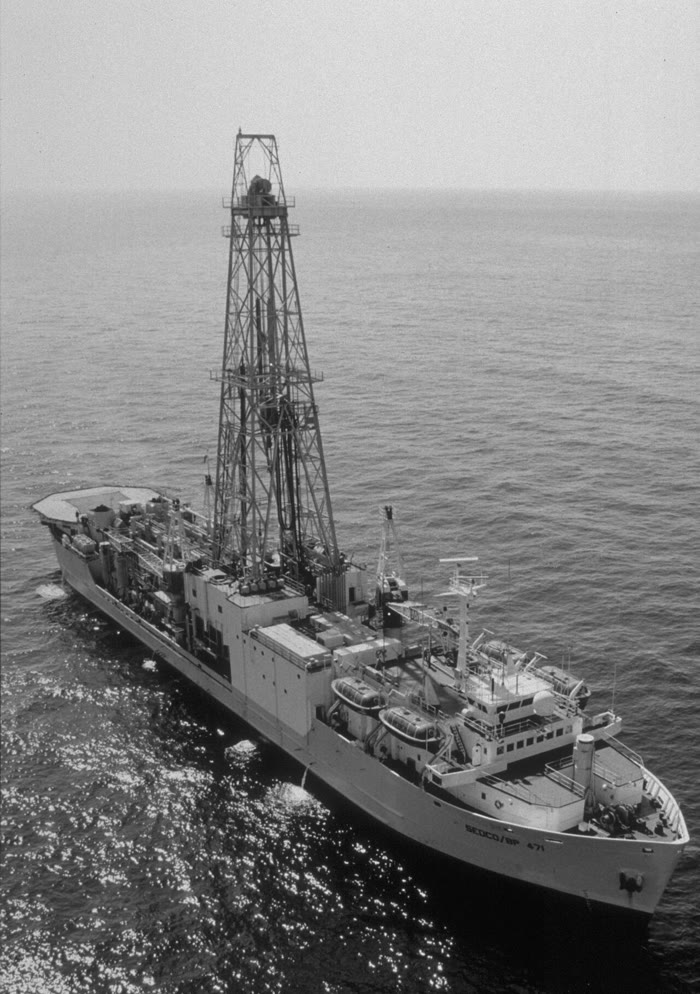
\includegraphics[width=0.36\linewidth]{images/book2/g11-odp-joides-resolution.jpg}

{\small 钻探船 \emph{JOIDES Resolution}，是继
\emph{Glomar Challenger} 之后的船只：高耸的塔架为其钻探井架，船上
载有超过 \qty{9000}{m} 的钻杆。照片：Ocean Drilling Program，Texas A\&M
University（公有领域）。}
\end{omfigure}
% ledger: photo:g11-joides, usgs:glomar

此后，数以千计的磁剖面与数百个钻孔已被
汇总成一幅整个大洋海底的年龄图。

\begin{omfigure}
\begin{tikzpicture}
\begin{axis}[ommap, width=\linewidth, xtick=\empty, ytick=\empty, grid=none,
    axis background/.style={}, clip=true, name=map]
  \addplot graphics[xmin=-180, xmax=180, ymin=-90, ymax=90] {figdata/out/grade-11-seafloor_age.png};
  \addplot[black!60, line width=0.15pt] table {figdata/out/shared-geo-land.dat};
\end{axis}
\begin{axis}[at={(map.south)}, anchor=north, yshift=-0.35cm, scale only axis, width=0.55\linewidth, height=0.32cm,
    xmin=0, xmax=200, ymin=0, ymax=1, axis y line=none, axis x line*=bottom,
    xtick={0,20,...,180}, tick label style={font=\scriptsize},
    xlabel={海底年龄（百万年）；灰色：无海底}, label style={font=\scriptsize},
    enlargelimits=false]
  \addplot graphics[xmin=0, xmax=200, ymin=0, ymax=1] {figdata/out/grade-11-seafloor_age-bar.png};
\end{axis}
\end{tikzpicture}

{\small 海底的年龄。最年轻的（红色）位于洋脊沿线，其
年龄向两侧远离洋脊方向逐渐增大；最古老的洋底（蓝色和紫色）位于
海洋边缘，紧邻大陆并沿海沟分布。
数据：Seton 等人（2020），以 1 度网格计；陆地轮廓：Natural
Earth。}
\end{omfigure}
% ledger: data:b2-seafloor-age, data:ne-land (map computed in figdata/grade-11/seafloor_age.py)

该图一次性印证了上述所有结论。沿每条洋脊，海底都很年轻，
其年龄向两侧对称增大。没有任何洋底老于
约 1.9 亿年：最古老的洋底位于西太平洋及
北美洲东海岸外（地中海东部的几个小盆地另行计算）。
洋底的平均年龄约为
6400 万年，其中约四分之三的洋底年龄小于 100
百万年——而大陆上保存着远为古老的岩石。
洋底之所以年轻，是因为它不断在洋脊处生成，并
如赫斯所指出的，在别处被消亡。其位置将
在\cref{ch:g11:subduction-zones}中讨论。
% ledger: data:b2-seafloor-age (oldest_open_myr 192.5, share_younger_100 0.76 in figdata/grade-11/seafloor_age.py), seton:mean-age, usgs:hess

\section{练习}

\begin{exercise}[$\star$]\label{exo:g11:drift-to-spreading:1}
定义\omterm{def:g11:drift-to-spreading:spreading}{海底扩张}。洋脊的\omterm{def:g11:drift-to-spreading:spreading-rate}{全扩张速率}与
半扩张速率有何区别？
\end{exercise}

\begin{exercise}[$\star$]\label{exo:g11:drift-to-spreading:2}
为什么熔岩只有冷却到
约 \qty{580}{\celsius} 以下时，才会记录地球磁场的方向？若
岩石之后被加热到 \qty{700}{\celsius}，该记录会发生什么变化？
\end{exercise}

\begin{exercise}[$\star$]\label{exo:g11:drift-to-spreading:3}
回声测深仪在发出脉冲后，经过 \qty{5.2}{s} 才接收到回声。
取海水中的声速为 \qty{1500}{m/s}，求
海底的深度。
\end{exercise}

\begin{exercise}[$\star$]\label{exo:g11:drift-to-spreading:4}
对照本章的极性时间尺度：当前的\omterm{def:g11:drift-to-spreading:reversal}{正极性}时段
已持续多久？Jaramillo 事件持续了多久？
最近 5 百万年内发生了多少次倒转？
\end{exercise}

\begin{exercise}[$\star$]\label{exo:g11:drift-to-spreading:5}
洋中脊的总长约为 \qty{65000}{km}，地球的周长
约为 \qty{40000}{km}。洋脊的长度相当于绕地球
多少圈？
\end{exercise}

\begin{exercise}[$\star\star$]\label{exo:g11:drift-to-spreading:6}
在某条磁剖面上，布容与松山时段之间的界线
（78 万年）位于距洋脊轴 \qty{20}{km} 处。求
每年以厘米计的半速率和全速率。
\end{exercise}

\begin{exercise}[$\star\star$]\label{exo:g11:drift-to-spreading:7}
在另一条剖面上，高斯–吉尔伯特界线（358 万年）
位于轴线以西 \qty{45}{km}、以东 \qty{44}{km} 处。求两侧的半速率
和全速率。扩张是否对称？
\end{exercise}

\begin{exercise}[$\star\star$]\label{exo:g11:drift-to-spreading:8}
1968 年钻探的第 19 站位于距大西洋中脊轴
\qty{990}{km} 处。取半速率为每年 \qty{1.9}{cm}，预测该处
海底的年龄，并与其最古老沉积物的 4900 万年
相比较。
\end{exercise}

\begin{exercise}[$\star\star$]\label{exo:g11:drift-to-spreading:9}
某洋脊的半扩张速率为每年 \qty{2}{cm}。利用本章的时间尺度，
求各界线距轴线的距离，界线年龄为 0.78、
0.99、1.07、1.77 和 1.95 百万年，并在一侧画出条带，
\omterm{def:g11:drift-to-spreading:reversal}{正极性}用黑色表示。
\end{exercise}

\begin{exercise}[$\star\star$]\label{exo:g11:drift-to-spreading:10}
洋底的平均年龄约为 6400 万年，地球的年龄
约为 \num{4.6} 十亿年。这一年龄占地球年龄的几分之几？
它支持赫斯的哪一论据？
\end{exercise}

\begin{exercise}[$\star\star$]\label{exo:g11:drift-to-spreading:11}
借助示意图解释：为什么洋脊一侧的磁条带图案
与另一侧的图案互为镜像？什么会破坏
这种对称性？
\end{exercise}

\begin{exercise}[$\star\star\star$]\label{exo:g11:drift-to-spreading:12}
假设全长 \qty{65000}{km} 的洋脊，平均\omterm{def:g11:drift-to-spreading:spreading-rate}{全扩张速率}
为每年 \qty{5}{cm}。
\begin{enumerate}
  \item 它们每年生成的新洋底面积是多少，单位为 \unit{km^2}？
  \item 洋底的面积约为 \qty{2.9e8}{km^2}。洋脊
        需要多长时间才能生成这么大的面积？
  \item 与最古老的洋底（约 1.9 亿年）相比较。
        洋底在生成的同时，必须以同样快的速度发生什么？
\end{enumerate}
\end{exercise}

\begin{exercise}[$\star\star\star$]\label{exo:g11:drift-to-spreading:13}
Jaramillo 事件发生于 \num{0.99} 至 107 万年前。
求其条带在半速率为每年 \qty{1.25}{cm} 的洋脊两侧的宽度，
以及在半速率为每年 \qty{7.5}{cm} 的洋脊两侧的宽度。被磁化的
岩石位于海面以下约 \qty{3}{km} 处。解释为什么该事件在本章的快速剖面上清晰可见，
而在慢速剖面上几乎不可见。
\end{exercise}

\begin{exercise}[$\star\star\star$]\label{exo:g11:drift-to-spreading:14}
在 1968 年的钻探站位中，第 16 站的沉积物厚 \qty{176}{m}，其海底
年龄约为 1100 万年；第 20 站仅厚 \qty{72}{m}，
海底约 6700 万年。求每个站位沉积物
堆积的平均速率，单位为米每百万年。沉积物
的厚度能否用来确定海底的年龄？若不能，则应改用什么？
\end{exercise}

\begin{exercise}[$\star\star\star$]\label{exo:g11:drift-to-spreading:15}
在穿过洋脊的剖面上，年龄为 258.1 万年的边界位于
轴线以西 \qty{58}{km}、以东 \qty{70}{km} 处。
\begin{enumerate}
  \item 分别计算两侧的半扩张速率与\omterm{def:g11:drift-to-spreading:spreading-rate}{全扩张速率}。
        \item 轴线以东的\omterm{def:g11:drift-to-spreading:spreading}{海底扩张}速度快于以西。
        按这些速率，经过 1000 万年后，
        该年龄的海底在两侧各距轴线多远？
        \item 解释为什么两条界线之间的距离可给出\omterm{def:g11:drift-to-spreading:spreading-rate}{全扩张速率}，
        即使扩张不对称也是如此。
\end{enumerate}
\end{exercise}

\section{问题：南大西洋的年龄}

\begin{problem}[{周末问题——用三种方法为一个大洋定年}]
\label{pb:g11:drift-to-spreading:1}
% ledger: dsdp3:table5, dsdp3:rate, data:b2-seafloor-age, earth:Rmean, ics:base.Cretaceous
% (values computed in figdata/grade-11/sediment_ages.py and seafloor_age.py)
1968 年，\emph{Glomar Challenger} 号钻探船在
南纬 \ang{30} 附近穿越大西洋中脊，共钻了七个钻孔。表中给出每个站位
的距洋脊轴线距离、玄武岩上最老沉积物的年龄，
（据化石确定），以及在其下方已识别磁条带时，该磁条带的
年龄，单位为百万年。

\begin{center}
\small
\begin{tabular}{|c|c|c|c|}
\hline
站位 & 距轴线距离（\unit{km}） & 最老沉积物年龄 & 磁条带年龄 \\ \hline
16 & 191 & 11 & 9 \\ \hline
15 & 380 & 24 & 21 \\ \hline
18 & 506 & 26 & --- \\ \hline
17 & 643 & 33 & --- \\ \hline
14 & 727 & 40 & 38.5 \\ \hline
19 & 990 & 49 & 53 \\ \hline
20 & 1270 & 67 & 71 \\ \hline
\end{tabular}

{\small 数据来源：Deep Sea Drilling Project，第 3 航次（1970）；磁条带年龄
取其所给范围的中点。}
\end{center}

\begin{center}
\begin{tikzpicture}
\begin{axis}[omrecord, width=0.82\linewidth, height=5.0cm, xmin=-50, xmax=16, ymin=0, ymax=140,
  xlabel={沿南纬 \ang{30} 的经度（度；负值为西）}, ylabel={年龄（百万年）},
  tick label style={font=\small}, label style={font=\small}, clip=false]
\addplot[omDef, line width=0.8pt] table[x=lon, y=age] {figdata/out/grade-11-seafloor_age-profile.dat};
\draw[omRidge, densely dashed] (axis cs:-13.8,0) -- (axis cs:-13.8,140);
\node[font=\scriptsize, text=omRidge, anchor=south] at (axis cs:-13.8,140) {洋脊轴线};
\fill (axis cs:-47.4,125.1) circle (1.5pt);
\node[font=\scriptsize, anchor=south west, inner sep=2pt] at (axis cs:-47.6,126) {南美洲};
\node[font=\scriptsize, anchor=north west, align=left] at (axis cs:14.2,135) {非洲};
\fill (axis cs:13.8,129.8) circle (1.5pt);
\end{axis}
\end{tikzpicture}

{\small 沿南纬 \ang{30} 纬线的洋底年龄，自
南美洲至非洲；曲线终止于洋底与
各大陆相接之处。数据来源：Seton 等（2020）。}
\end{center}

\medskip
\noindent\textbf{第一部分——钻探站位。}
\begin{enumerate}
  \item 哪个站位离洋脊最近，哪个最远？它们的
        年龄如何比较？
  \item 为什么玄武岩上最老沉积物的年龄接近
        玄武岩本身的年龄？它略老一些还是
        略年轻一些？
  \item 对每个站位，计算其距离与最老沉积物年龄之比，
        单位为千米每百万年。
  \item 求这七个比值的平均值，并将其换算为厘米
        每年。
  \item 站位 17 和 18 位于洋脊以东，其余位于以西。
        东侧站位是否与西侧遵循相同的趋势？这对
        \omterm{def:g11:drift-to-spreading:spreading}{海底扩张}说明了什么？
\end{enumerate}

\medskip
\noindent\textbf{第二部分——由沉积物求速率。}
\begin{enumerate}[resume]
  \item 若海底以恒定半扩张速率 $u$ 扩张，
        海底的年龄 $t$ 与其距轴线距离 $d$ 有何关系？
  \item 通过原点且最佳拟合各点的直线，其斜率为
        $u = \sum d\,t / \sum t^2$。对这七个站位，
        $\sum d\,t = \num{208276}$，$\sum t^2 = \num{10952}$（单位为
        千米与百万年）。求 $u$，以千米每百万年为
        单位，并以厘米每年表示。
  \item 求该纬度处南大西洋的\omterm{def:g11:drift-to-spreading:spreading-rate}{全扩张速率}
        是多少？
  \item 考察队的科学家写道：该速率“每年略低于
        \qty{2}{cm}”。你是否同意？
  \item 按此速率，预测站位 20 处海底的年龄，并与
        其最老沉积物的年龄进行比较。
\end{enumerate}

\medskip
\noindent\textbf{第三部分——由磁条带求速率。}
\begin{enumerate}[resume]
  \item 仅由站位 16（\qty{191}{km}，磁条带年龄 900 万年），
        计算一个半扩张速率。
  \item 仅由站位 20（\qty{1270}{km}，磁条带年龄 7100 万年），
        计算一个半扩张速率。
  \item 对具有磁条带年龄的五个站位，$\sum d\,t = \num{180329}$，
        $\sum t^2 = \num{9854}$。求最佳半扩张速率。
  \item 由化石与由磁条带得出的速率相差百分之几？
        两种方法是否一致？
  \item 两种年龄由完全不同的方法得出，为什么
        这一点十分重要？
\end{enumerate}

\medskip
\noindent\textbf{第四部分——直到大洋的边缘。}
\begin{enumerate}[resume]
  \item 沿南纬 \ang{30}，洋脊轴线位于经度
        \ang{13.8} 西，洋底在非洲一侧止于
        \ang{13.8} 东处。两者相隔多少度经度？
  \item 设球半径为 \qty{6371}{km}，经度一度的长度为
        $\qty{111.2}{km} \times \cos(\text{纬度})$。求
        南纬 \ang{30} 处经度一度的长度，以及
        轴线到非洲一侧洋底边缘的距离。
  \item 若海底始终以第二部分中的速率扩张，
        则边缘处的海底形成于多久以前？
  \item 年龄图通过磁条带给古老海底定年，给出
        边缘处为 1.3 亿年。由此得出的
        平均半扩张速率是多少？大洋早期张开的速度
        略快还是略慢于最近 6600 万年的张开速度？
  \item 归纳：南纬 \ang{30} 处非洲一侧最古老洋底的
        年龄是多少？白垩纪约始于 1.43 亿年前，
        南大西洋在该处开始张开，
        发生在哪一纪？
\end{enumerate}
\end{problem}
